\documentclass[addpoints,12pt]{exam}

\usepackage[locale=FR, group-digits=all, group-separator=\ , group-minimum-digits=4, per-mode = symbol]{siunitx}
\usepackage[margin=1.5cm]{geometry}
\usepackage{mdframed}
\usepackage{tikz}
\usepackage{frenchmath}
\DeclareSIUnit{\litre}{\ell}
\usepackage{amsmath}
\usepackage{eurosym}
\DeclareSIUnit{\EURO}{\text{\euro}}

\newcommand{\titre}[1]{%
    % #1 : numéro du DS
    \begin{center}%
        \Huge{DS n°#1}%    
    \end{center}%
}

\begin{document}

\titre{1}

\qformat{\textbf{\underline{Exercice \thequestion : }} \hfill [\thepoints]}
\begin{questions}
    \question[4] On donne les deux programmes de calcul suivants :

    \begin{center}
        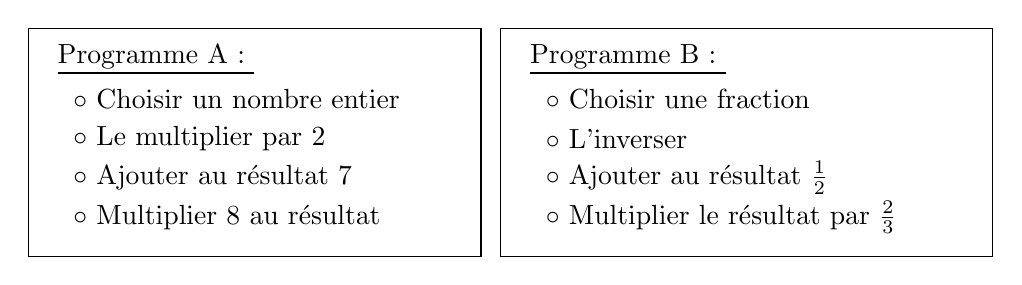
\begin{tikzpicture}
            \draw (-0.25,0.4) rectangle (5.5,-2.5);
            \node[anchor=west] at (0,0) {\underline{Programme A : }};
                \node[anchor=west] at (0.2,-0.5) { $\circ$ Choisir un nombre entier};
                \node[anchor=west] at (0.2,-1.0) { $\circ$ Le multiplier par 2};
                \node[anchor=west] at (0.2,-1.5) { $\circ$ Ajouter au résultat 7};
                \node[anchor=west] at (0.2,-2.0) { $\circ$ Multiplier 8 au résultat};
            \draw (5.75,0.4) rectangle (12,-2.5);
            \node[anchor=west] at (6,0) {\underline{Programme B : }};
                \node[anchor=west] at (6.2,-0.5) { $\circ$ Choisir une fraction};
                \node[anchor=west] at (6.2,-1.0) { $\circ$ L'inverser};
                \node[anchor=west] at (6.2,-1.5) { $\circ$ Ajouter au résultat $\frac{1}{2}$};
                \node[anchor=west] at (6.2,-2.0) { $\circ$ Multiplier le résultat par $\frac{2}{3}$};
        \end{tikzpicture}
    \end{center}

    \begin{parts}
        \part En choisissant $3$ dans le programme de calcul A, vérifier que l'on trouve bien $104$.
        \part En choisissant $\dfrac{5}{4}$ dans le programme de calcul B, vérifier que l'on trouve bien $\dfrac{26}{30}$.
        \part En choisissant $1$ dans le programme A et $\dfrac{2}{215}$ dans le programme B, on trouve le même résultat. Montrer que cela est vrai en faisant les deux calculs.
    \end{parts}

    \question[6]
    \begin{parts}
        \part Dans le triangle $ABC$ rectangle en $B$, $AB = \qty{3,1}{\centi\metre}$ et $BC = \qty{6,2}{\centi\metre}$. Déterminer la distance $AC$.
        \part Une échelle est posée sur un mur. Elle mesure \qty{5,5}{\metre}. Elle est posée au sol à \qty{2}{\metre} du mur.
        \begin{subparts}
            \subpart Faire un schéma, et expliquer pourquoi on peut modéliser le problème par un triangle rectangle.
            \subpart Posée de cette manière, quelle hauteur l'échelle permettra d'atteindre ?
        \end{subparts}
    \end{parts}

    \question[4]
    Pierre va acheter 2 baguettes et 3 éclairs aux chocolats à la boulangerie.\\
    Une baguette coûte \qty{1,20}{\EURO} et un éclair au chocolat coûte \qty{2,20}{\EURO}. 

    \begin{parts}
        \part Quel calcul faut-il faire pour trouver le prix de l'ensemble de ce qu'il a acheté ?
        \part Faire le calcul, et conclure.
    \end{parts}

    \question[4]
        Un pavé droit en argent a les dimensions suivants : $L = \qty{7}{\centi\metre}$, $\ell = \qty{3}{\centi\metre}$, $h = \qty{2}{\centi\metre}$. \\
        La masse volumique de l'argent est \qty{10,50}{\gram\per\centi\metre\cubed}. Calculer la masse de ce pavé droit.

    \question[2] Donner le 278ème chiffre après la virgule de $\dfrac{16,3}{999}$.
\end{questions}

\vfill
\begin{center}
    \gradetable[h][questions]
\end{center}

\end{document}